\chapter{Introdução}
\label{cha:introducao}

Contorno pode ser definido como o perfil, desenho ou formato de um
objeto. Pode ser bidimensional e associar altura a comprimento,
largura ou tempo. Em música contornos podem ser associados a altura,
densidade, ritmo, complexidade rítmica, homogeneidade orquestral,
amplitude de harmônicos, intensidade, etc. Contornos melódicos estão
relacionados com movimento de altura de notas em função do tempo.

O estudo de contornos é importante porque, assim como conjuntos de
notas e motivos, contornos podem ajudar a dar coerência a uma obra
musical. Eles representam estruturas musicais manipuláveis através de
várias operações como inversão e retrogradação, e podem ser abordados
tanto do ponto de vista da análise quanto da composição.

Apesar da possível coerência musical proporcionada por contornos e das
operações fornecidas por teorias de contornos, ainda assim são
escassos estudos sistemáticos do uso dessas operações de contorno e de
suas combinações na composição musical. Acreditamos ser necessário um
estudo e experimentação dessas operações na composição.

Neste trabalho fazemos a revisão de teorias desenvolvidas para o
estudo de contornos, criamos um programa de computador para
processamento de contornos e apresentamos a análise e partitura da
obra \obra{}, composta com base em combinações de operações de
contornos.

\section{Objetivos e justificativa}
\label{sec:objet-e-just}

O presente trabalho tem como principais objetivos a composição de uma
obra musical com base em combinações de operações de contornos e a
produção do seu memorial. O instrumental da obra é um quinteto de
madeiras e a duração é de aproximadamente 11 minutos.

São objetivos secundários deste trabalho:

\begin{enumerate}
\item Desenvolvimento de um programa de computador para processamento
  de operações de contornos melódicos.
\item Entendimento do mapeamento de contornos para elementos
  musicais/composicionais.
\item Compreensão do estado de arte de contornos melódicos.
\end{enumerate}

O uso sistemático de contornos melódicos tanto para geração de
material composicional quanto como determinante composicional é um
assunto carente de literatura. Este estudo pode elevar o estado de
arte das teorias de contornos e contribuir com novas ferramentas para
a área de Composição.

\section{Metodologia}
\label{sec:metodologia}

Para a realização deste trabalho cumprimos as seguintes atividades:

\begin{enumerate}
\item Revisão de literatura sobre contornos melódicos

\item Mapeamento de contornos para elementos musicais

  Trata-se da representação de elementos musicais como altura e
  duração para contornos. Envolveu o estudo das particularidades de
  tais elementos como representação numérica de notas, intervalos e
  ritmo, bem como estudo de possíveis operações de contornos.

\item Composição de estudos para experimento de possibilidades com
  contornos melódicos.

  Compomos duas peças para experimentar possibilidades com operações
  de contornos melódicos\footnote{Vide partituras destas peças nos
    anexos deste trabalho.}. A primeira---\opus{Como é que se preenche
    um contorno melódico? Op.3}---contém um único contorno melódico e
  operações de preenchimento deste contorno. A segunda---\opus{Bobó de
    legumes. Op.5}---contém também um único contorno e suas operações
  e concatenações. Com estes experimentos foi possível aprofundar a
  prática da composição de contornos antes de compor a obra final do
  mestrado.

\item Desenvolvimento de um programa de computador para processar
  operações com contornos melódicos (vide seção
  \ref{sec:goiaba-software-para}).

  Desenvolvemos um software que lida com contornos melódicos,
  operações e combinações. Ele retorna representações simbólicas e
  gráficas de operações de transposição, inversão, retrogradação e
  rotação de um dado contorno. Além disso ele permite a combinação de
  operações e sua concatenação. Este software ajudou no mapeamento e
  processamento de contornos melódicos no estudo do estado de arte, na
  composição dos experimentos, e na composição da obra final.
  
\item Composição da peça (vide capítulo \ref{cha:anal-da-obra}).

\item Escrita da dissertação
\end{enumerate}

\section{Estrutura da dissertação}
\label{sec:estr-da-diss}

Esta dissertação está organizada da seguinte maneira:

\begin{itemize}
\item Capítulo 1: identificação dos problemas abordados e objetivos
  deste trabalho
\item Capítulo 2: abordagem do estado de arte de contornos
\item Capítulo 3: descrição das ferramentas desenvolvidas e utilizadas
\item Capítulo 4: análise da obra \obra{}
\end{itemize}

\chapter{Estado de arte de contornos}
\label{cha:estado-de-arte-contornos}

Há diversas definições de contorno melódico na literatura
\cite{piston59:harmony,toch77:shaping,schonberg:fundamentals,adams76:melodic,marvin.ea87:relating,morris87:composition,clifford95:contour,beard03:contour},
sendo cada uma delas relacionada com o objetivo do trabalho de seu
autor. Para o presente estudo preferimos criar uma definição
própria. Dessa forma entendemos que contorno melódico é um conjunto
ordenado de alturas de notas (chamadas de pontos) cujo valor absoluto
é ignorado e somente o registro, que pode ser mantido ou variar
ascendente e descendentemente entre um ponto e outro, é
considerado.

Por exemplo, no fragmento da 5ª Sinfonia de Beethoven (figura
\ref{fig:5a-sinfonia}), ignoramos todas as alturas e intervalos,
consideramos que não há diferença de registro entre as três primeiras
notas, que a nota Mi$\flat$ tem registro mais grave que a nota Sol,
que a nota Fá tem registro mais agudo que a nota Mi$\flat$, e que a
nota Ré tem registro mais grave que a nota Fá. Estes movimentos
delineiam o contorno do fragmento.

\begin{figure}
  \centering
  \includegraphics{5a-sinfonia}
  \caption{Fragmento da 5ª Sinfonia de Beethoven}
  \label{fig:5a-sinfonia}
\end{figure}

A idéia de preservação de contornos e variação de intervalos entre
notas é encontrada em diferentes situações musicais. Há adequação de
notas à tonalidade em respostas tonais de fugas, em mudanças de modo
em peças do tipo tema e variações, e em \eng{leitmotifs} e idéias
fixas, citando apenas exemplos óbvios
\cite[p. 29]{morris87:composition}. Outras obras têm motivos cujos
intervalos são progressivamente expandidos ou contraídos, como por
exemplo ocorre no início da \opus{Música para Cordas, Percussão e
  Celesta}, de Béla Bartók.

Embora haja na literatura estudos sobre contornos associados a duração
\cite{beard03:contour}, não abordamos este aspecto neste
trabalho. Percebemos ao longo do processo que incluir a duração em
nosso estudo demandaria mais tempo do que o disponível e
inviabilizaria o projeto.

Neste estudo consideramos como operação de contorno todo tipo de
manipulação de um contorno. Dessa forma consideramos operações
procedimentos como inversão, retrogradação, expansão e subconjuntos de
contorno, bem como procedimentos da literatura de contornos como
matriz de comparação, classe de contorno, INT$_n$, e várias
outras. Estas operações fornecidas pelas teorias de contornos são
detalhadas na seção \ref{sec:teor-de-cont}.

Teorias de contornos foram desenvolvidas primariamente como técnicas
analíticas aplicáveis a composições atonais que não possuem as
características musicais típicas como frase, períodos, temas e
harmonia funcional, que dão coerência a composições tonais
\cite[p. 1]{beard03:contour}.

%% comentar o sucesso e o que foi achado de diferente nas análises de
%% friedmann, clifford e beard
Embora teorias de contorno não tenham surgido para análise de obras
tonais, a análise a partir da perspectiva dos contornos já se mostrou
eficiente também neste tipo de obra. Assim, além de obras de Schönberg
\cite{friedmann85:methodology} e Webern \cite{clifford95:contour},
sonatas para piano de Mozart \cite{beard03:contour} já foram
analisadas sob a ótica das teorias de contornos.

Contorno é um conjunto ordenado de elementos distintos, com ou sem
repetição, numerados de forma ascendente
\cite[p. 206]{morris93:directions}.

Um contorno pode ser interpretado como registro, dinâmica ou densidade
de acordes no tempo \cite[p. 206]{morris93:directions}
\cite[p. 22]{clifford95:contour}. Um dado contorno (4 3 5 6), por
exemplo, pode ser associado ao parâmetro registro com as notas Lá, Fá,
Si$\flat$ e Ré (figura \ref{fig:pitches-in-time}); pode ser associado
a densidades de acordes com acordes de duas, uma, quatro e sete notas
(figura \ref{fig:chord-densities-in-time}); ou pode ainda ser
associado aos graus de dinâmica \music{p}, \music{ppp}, \music{mf} e
\music{fff} (figura \ref{fig:dynamics-in-time}).

\begin{figure}
  \centering
  \subfloat[alturas no tempo]{
    \includegraphics[scale=1]{pitches-in-time}
    \label{fig:pitches-in-time}}
  \subfloat[densidade de acordes no tempo]{
    \includegraphics[scale=1]{chord-densities-in-time}
    \label{fig:chord-densities-in-time}}

  \subfloat[dinâmicas no tempo]{
    \includegraphics[scale=1]{dynamics-in-time}
    \label{fig:dynamics-in-time}}
  \caption{Contornos (4 3 5 6) não melódicos}
  \label{fig:non-melodic-contours}
\end{figure}

\section{Estudos de contorno em outras áreas da Música}
\label{sec:estudos-de-contorno}

Há estudos e aplicações de contornos melódicos também em outras áreas
da música como Etnomusicologia, Computação e Percepção Musical. Na
área da Etnomusicologia contornos são usados para representar e
classificar melodias populares \cite{adams76:melodic}. Na área da
Computação musical, especificamente, \eng{Music Information
  Retrieval}, contornos são utilizados em sistemas \eng{query by
  humming}---de busca em bases de dados a partir de melodias cantadas
\cite{ghias.ea95:query}.

No campo da percepção musical é reconhecido que ouvintes têm maior
acuidade na percepção de semelhança de contornos do que na semelhança
de alturas, e que o contorno melódico é um importante recurso para o
reconhecimento de melodias familiares \cite[p. 226,
136]{dowling.ea86:music}. Esta afirmação é endossada por experimentos
realizados por White \cite{white60:recognition}, e Dowling e Fujitani
\cite{dowling.ea71:contour} nos quais ouvintes foram submetidos ao
reconhecimento de versões de canções familiares que tinham ritmo e/ou
intervalos melódicos modificados e o contorno preservado.

%% talvez merge
%% que "outros elementos"?
Implicações do estudo de contornos na música do século XX são mais
significativas para os ouvintes do que para os compositores. Isto
porque a percepção de contornos é mais geral do que a percepção de
altura e dos outros elementos do universo da teoria atonal
\cite[p. 224]{friedmann85:methodology}.

A idéia de Hindemith sobre percepção de contornos é semelhante à dos
demais autores, embora o contexto em que se aplique seja o do estudo
da harmonia. De acordo com ele é mais fácil lembrar de sucessão
rítmica e de curvas de uma linha melódica do que de diferenças em
tensão entre harmonias \cite[p. 175]{hindemith41:craft}.

\section{Contorno como determinante composicional}
\label{sec:cont-como-determ}

Analisando obras de Anton Webern, Clifford concluiu que contorno pode
ser entendido como um determinante composicional. De acordo com ele
\citacaoinline{contour, in absence of other pervasive systems of pitch
  organization, represents a structural factor equal in significance
  to pitch or set class relations}{contorno, na falta de outros
  sistemas ocupantes de organização de altura, representa um fator
  estrutural igual em significado a relações de alturas ou de classes
  de conjuntos}{p. 157}{clifford95:contour}

No nível melódico relações de contorno podem associar segmentos de
contorno distintos entre dois ou mais segmentos. Neste nível contorno
pode contribuir com um processo de transformação melódica
\cite[p. 159]{clifford95:contour}.

\section{Teorias de contornos}
\label{sec:teor-de-cont}

Teorias que visam sistematizar o estudo de contornos dispõem de várias
operações para mapeamento e comparação de contornos
\cite{friedmann85:methodology,friedmann87:response,morris87:composition,morris93:directions,marvin.ea87:relating,clifford95:contour,polansky.ea92:possible,quinn97:fuzzy,beard03:contour}
\note{período fragmentado}.  A partir das idéias destas teorias é
possível, por exemplo, reconhecer semelhanças de registro entre as
duas melodias de quatro notas da figura \ref{fig:ly-cseg-5968}, cujo
contorno está representado graficamente na figura
\ref{fig:cseg-5968}. Estas semelhanças são identificadas apenas se
observamos os seus contornos. Outros exemplos de melodias de contornos
semelhantes podem ser vistos nas figuras \ref{fig:melodias-cseg} e
\ref{fig:graficos-cseg}.

\begin{figure}
  \centering
  \subfloat[melodias de contorno P(5 9 6 8)]{
    \includegraphics[scale=.9]{ly-5968}
    \label{fig:ly-cseg-5968}
  }
  \subfloat[melodias de contorno Q(5 7 6 8)]{
    \includegraphics[scale=.9]{ly-5768}
    \label{fig:ly-cseg-5768}
  }

  \subfloat[melodias de contorno R(3 0 5 1)]{
    \includegraphics[scale=.9]{ly-3051}
    \label{fig:ly-cseg-3051}
  }
  \caption{Melodias para diferentes contornos}
  \label{fig:melodias-cseg}
\end{figure}

\begin{figure}
  \centering
  \subfloat[contorno P(5 9 6 8)]{
    \includegraphics{c-5968}
    \label{fig:cseg-5968}
  }
  \subfloat[contorno Q(5 7 6 8)]{
    \includegraphics{c-5768}
    \label{fig:cseg-5768}
  }
  \subfloat[contorno R(3 0 5 1)]{
    \includegraphics{c-3051}

    \label{fig:cseg-3051}
  }
  \caption{Gráficos de contornos}
  \label{fig:graficos-cseg}
\end{figure}

A música pode ser visualizada em diferentes espaços, como de altura e
de contorno \cite{morris87:composition}. O espaço de contorno
(\tr{c-space}) é uma abstração de espaço musical que consiste em
elementos organizados do grave para o agudo desconsiderando os
intervalos exatos entre eles. Leva-se em conta apenas a relação entre
os registros dos elementos. O espaço de contorno pode ser entendido
como um grande conjunto de alturas de contorno (\tr{c-pitch}).

Cada conjunto de alturas de contorno contido em um espaço de contorno
é chamado de segmento de contorno (\tr{cseg})\footnote{Trata-se de uma
  idéia semelhante à da geometria, de reta e segmento de reta, onde o
  espaço de contorno seria análogo à reta, e o segmento de contorno ao
  segmento de reta.}. Estes segmentos de contornos podem conter
elementos contíguos ou não contíguos do espaço de
contorno. Subconjuntos de segmentos de contornos são chamados
\tr{csubseg}. Para uma simplificação terminológica, neste trabalho nos
referimos a segmento de contorno com o termo genérico ``contorno''. A
figura \ref{fig:c-space} contém três exemplos de um mesmo espaço de
contorno de 10 alturas de contorno enumeradas do mais grave (0) para o
mais agudo (9). Na figura \ref{fig:c-space5968} o espaço de contorno
contém o contorno P, com as alturas de contorno 5, 9, 6 e 8. Na figura
\ref{fig:c-space7420} o espaço de contorno contém o contorno M, com
alturas de contorno 7, 4, 2 e 0. Ainda nesta figura o contorno M
contém o subconjunto de contorno O, com alturas de contorno 4 e 2. Por
último, na figura \ref{fig:c-space564} o espaço de contorno contém o
contorno N, com as alturas de contorno não adjacentes 5, 6 e 4.

\begin{figure}
  \centering
  \subfloat[contorno P]{
    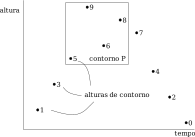
\includegraphics[scale=1]{cspace-5968}
    \label{fig:c-space5968}
  }
  \subfloat[contorno M e subconjunto O]{
    \includegraphics[scale=1]{cspace-7420}
    \label{fig:c-space7420}
  }

  \subfloat[contorno N]{
    \includegraphics[scale=1]{cspace-564}
    \label{fig:c-space564}
  }
  \caption{Espaço de contorno com diferentes contornos e subconjunto
    de contorno}
  \label{fig:c-space}
\end{figure}

Os contornos são representados por letras maiúsculas e têm seus
elementos representados por numerais subscritos, como A$_3$. Estes
numerais indicam a posição destes elementos em ordem temporal
\cite{marvin.ea87:relating}. Por exemplo, um contorno P de quatro
elementos tem a seguinte configuração: P(P$_0$ P$_1$ P$_2$
P$_3$). Dessa forma, dado um contorno P(5 9 6 8), P$_0$ é igual a 5,
P$_1$ é igual a 9 e P$_2$ é igual a 6.

Operações como retrogradação e rotação são semelhantes às realizadas
com alturas de notas. Um contorno P(5 9 6 8) tem retrógrado RP(8 6 9
5), rotação de fator 1 Rot-1P(9 6 8 5), rotação de fator 2 Rot-2P(6 8
5 9) e assim por diante. As representações gráficas dessas operações
podem ser vistas na figura \ref{fig:operacoes-simples}. A expansão de
intervalos consiste na multiplicação dos intervalos entre cada altura
de contorno por um dado fator. Por exemplo, a expansão de fator 2 do
contorno (5 9 6 8) é (5 13 7 11).

\begin{figure}
  \centering
  \subfloat[Contorno P]{
    \includegraphics{c-5968}
    \label{fig:operacoes-p}
  }
  \subfloat[Inversão de P]{
    \includegraphics{c-4031}
    \label{fig:operacoes-ip}
  }
  \subfloat[Retrógrado de P]{
    \includegraphics{c-8695}
    \label{fig:operacoes-rp}
  }
  \subfloat[Retrógrado da inversão de P]{
    \includegraphics{c-1304}
    \label{fig:operacoes-ip}
  }

  \subfloat[Rotação 1 de P]{
    \includegraphics{c-9685}
    \label{fig:operacoes-rr1}
  }
  \subfloat[Rotação 2 de P]{
    \includegraphics{c-6859}
    \label{fig:operacoes-rr2}
  }
  \subfloat[Rotação 3 de P]{
    \includegraphics{c-8596}
    \label{fig:operacoes-rr3}
  }
  \caption{Representação gráfica de operações simples com contorno P(5
  9 6 8)}
  \label{fig:operacoes-simples}
\end{figure}

A operação de inversão de um contorno P de ordem $q$ é representada
por IP, e é matematicamente calculada por IP$_n=(q-1-P_n)$. Portanto,
dado um contorno P(5 9 6 8), de ordem 10, IP$_0=(10-1-P_0)$. Logo,
IP$_0=4$. Aplicando-se a mesma idéia aos outros elementos chegamos ao
contorno IP(4 0 3 1) (figura \ref{fig:operacoes-simples}). É possível
ainda relacionar a inversão entre elementos através da matriz de
comparação. Calcula-se esta inversão com a operação
$COM(P_a,P_b)=-COM(IP_a,IP_b)$.

Relações de similaridade \cite{marvin.ea87:relating} são analisadas
com operações como comparação, matriz de comparação e classe de
contorno.

A operação de comparação \tr{COM(a,b)} retorna a diferença de registro
entre dois elementos $a$ e $b$, ou seja, informa se um elemento é mais
agudo, mais grave ou de mesma altura que outro. O valor da operação de
comparação é o sinal ``$+$'' se $b$ é maior que $a$; ``$-$'' se $b$ é
maior que $a$; e ``$0$'' se $b$ é igual a $a$. Por exemplo, no
contorno P(5 9 6 8), o valor de $COM(P_0,P_1)$ é o sinal ``$+$'', o de
$COM(P_1,P_2)$ é ``$-$'', e o valor de $COM(P_3,P_0)$ é o sinal
``$+$''. Esta medida de comparação pode ser invertida de modo que a
comparação entre dois elementos é igual ao inverso da comparação
destes elementos em ordem reversa. Esta idéia pode ser melhor
entendida observando-se a equação $COM(a,b)=-COM(b,a)$.

A matriz de comparação (COM-Matrix) é bidimensional e compara um
contorno com ele próprio. Esta matriz mostra os resultados da operação
de comparação para todas as alturas de contorno de um contorno. A
tabela \ref{fig:matriz-5968} contém a matriz de comparação de um
contorno P(5 9 6 8). As matrizes de comparação dos exemplos já vistos
na figura \ref{fig:graficos-cseg} podem ser vistos na tabela
\ref{fig:matriz-exemplos}.

\begin{figure}
  \centering
  \subfloat[contorno P(5 9 6 8)]{
    \begin{tabular}{c|cccc}
      & $5$ & $9$ & $6$ & $8$ \\
      \hline
      $5$ & $0$ & $+$ & $+$ & $+$ \\
      $9$ & $-$ & $0$ & $-$ & $-$ \\
      $6$ & $-$ & $+$ & $0$ & $+$ \\
      $8$ & $-$ & $+$ & $-$ & $0$
    \end{tabular}
    \label{fig:matriz-5968}
  }
  \qquad
  \subfloat[contorno Q(5 7 6 8)]{
    \begin{tabular}{c|cccc}
      & $5$ & $7$ & $6$ & $8$ \\
      \hline
      $5$ & $0$ & $+$ & $+$ & $+$ \\
      $7$ & $-$ & $0$ & $-$ & $+$ \\
      $6$ & $-$ & $+$ & $0$ & $+$ \\
      $8$ & $-$ & $-$ & $-$ & $0$
    \end{tabular}
    \label{fig:matriz-5768}
  }
  \qquad
  \subfloat[contorno R(3 0 5 1)]{
    \begin{tabular}{c|cccc}
      & $3$ & $0$ & $5$ & $1$ \\
      \hline
      $3$ & $0$ & $-$ & $+$ & $-$ \\
      $0$ & $+$ & $0$ & $+$ & $+$ \\
      $5$ & $-$ & $-$ & $0$ & $-$ \\
      $1$ & $+$ & $-$ & $+$ & $0$
    \end{tabular}
    \label{fig:matriz-3051}
  }
  \caption{Exemplos de matriz de comparação}
  \label{fig:matriz-exemplos}
\end{figure}

As diagonais superiores paralelas à diagonal principal zero da matriz
de comparação são chamadas de INT$_n$, onde $n$ é o número da
diagonal: 1 para a superior mais próxima da diagonal zero, 2 para a
seguinte, 3 para a posterior e assim por diante.

A diagonal INT$_1$ traz comparações de registros entre elementos
adjacentes do contorno. Em P(5 9 6 8), por exemplo, INT$_1=(+ - +)$,
ou seja, o movimento melódico é ascendente entre 5 e 9, descendente
entre 9 e 6, e ascendente entre 6 e 8. Esta comparação é feita também
com uma operação conhecida como série de contornos adjacentes
(\tr{CAS})\footnote{Em teorias de contornos não há consenso em relação
  a terminologia. Dessa forma há idéias semelhantes com nomes
  diferentes, como INT$_1$ e Série de contornos adjacentes
  \cite{friedmann87:response}. A série de contornos adjacentes de
  Friedmann, por exemplo, seria entendida por Morris como uma série de
  alturas de contorno adjacentes.}. A tabela \ref{tab:int-contornos}
traz as INT$_n$ dos contornos (5 9 6 8), (5 7 6 8) e (3 0 5 1), cujas
matrizes são apresentadas na figura \ref{fig:matriz-exemplos}.

\begin{table}
  \centering
  \begin{tabular}{r|ccc}
    Contorno & INT$_1$ & INT$_2$ & INT$_3$ \\
    \hline
    (5 9 6 8) & (+ - +) & (+ -) & (+) \\
    (5 7 6 8) & (+ - +) & (+ -) & (+) \\
    (3 0 5 1) & (- + -) & (+ +) & (-)
  \end{tabular}
  \caption{Exemplos de INT$_n$}
  \label{tab:int-contornos}
\end{table}

A classe de contorno (\tr{CC}) é uma operação importante para a
verificação de similaridade entre contornos. Obtém-se classe de
contorno numerando-se ordenadamente todas as alturas de contorno de
$0$ a $(n-1)$, sendo $n$ o número total de alturas de contorno do
contorno. Uma classe de contorno engloba todos os contornos
considerados equivalentes. Dois ou mais contornos são considerados
equivalentes quando geram uma mesma matriz de comparação, ou seja,
quando mantêm a mesma estrutura de registro entre suas notas. Dessa
forma, dado um contorno P(5 9 6 8), são considerados seus equivalentes
os contornos (1 5 2 3), (0 10 4 7), (0 3 1 2) e muitos outros. Todos
eles têm (0 3 1 2) como forma normal e classe de contorno.

Os Intervalos de Contorno (\tr{CI}) representam as relações entre
alturas de contorno de uma classe de contorno e podem ser entendidos
de duas formas: guardando o valor entre as alturas de contorno
\cite{friedmann85:methodology}, ou guardando apenas a direção, mas não
o valor da diferença entre as alturas de contorno
\cite{morris93:directions}. Por exemplo, para um mesmo contorno P(0 3
1 2), o intervalo de contorno entre $P_1$ e $P_2$ para Friedmann é -2,
e para Morris, ``$-$''.

O Vetor de Intervalos de Contornos (\tr{CIA}) descreve a freqüência de
cada tipo de intervalo de contorno em uma classe de contorno. Por
exemplo, o contorno P(0 3 1 2) tem vetor de intervalos de contornos
(2,1,1/1,1,0). Os dígitos da esquerda da barra representam os
intervalos de contorno ascendentes em ordem crescente, e os dígitos da
direita os intervalos de contorno descendentes em ordem crescente de
valor absoluto. \cite{friedmann85:methodology}. Os Vetores de classe
de contorno (\tr{CCVI} e \tr{CCVII}), de dois dígitos cada um,
refletem os movimentos ascendentes e descendentes de um contorno e são
calculados a partir dos intervalos de contorno ascendentes e
descendentes.

A redução de contornos é possível a partir de dois diferentes
algoritmos \cite{adams76:melodic,morris93:directions}. O algoritmo de
Adams, criado para definir uma tipologia de contornos, reduz uma
melodia inteira a apenas quatro alturas de contorno\footnote{Adams
  utiliza uma terminologia diferenciada da que apresentamos aqui.}: a
primeira altura, a última, a mais aguda e a mais grave. O algoritmo de
Morris, processado em várias etapas, reduz a melodia através da
observação de mudanças de direção entre segmentos adjacentes e
eliminação de alturas de contorno.

A tipologia de Adams considera a inclinação entre as quatro alturas de
contorno extremas e compreende 15 tipos de contornos melódicos, como
se vê na figura \ref{fig:adams-typology}. A inclinação (ou
\eng{slope}) entre a nota inicial e final é indicada por $S1$ ($I >
F$), $S2$ ($I = F$) e $S3$ ($I < F$). A mudança de direção (ou
\eng{deviation}) é indicada por $Dø$ (sem mudança de direção), $D1$
(se H ou L são diferentes de I ou F) e $D2$ (se H e L são diferentes
de I e F). A ordem entre as mudanças de direção, chamada
\eng{reciprocal}, é indicada por $R1$ (H antes de L) e $R2$ (L antes
de H) \cite{adams76:melodic}.

\begin{figure}
  \centering
  \includegraphics[scale=.6]{adams-typology}
  \caption{Tipologia de contornos de Charles Adams}
  \label{fig:adams-typology}
\end{figure}

\chapter{Ferramentas}
\label{cha:ferramentas}

Para este trabalho desenvolvi ferramentas computacionais exclusivas
como o Goiaba, um software para processar contornos, bem como utilizei
sistema de controle de versão e softwares para edição profissional de
texto e partituras.

\section{Goiaba, um software para processar contornos}
\label{sec:goiaba-software-para}

O \goiaba{} é desenvolvido na linguagem Common
Lisp\footnote{Disponível em \url{cliki.net/CLiki}} com o compilador
SBCL\footnote{Disponível em \url{sbcl.org}}.
%% falar sobre as classes do goiaba
A classe \texttt{ponto} define pontos cartesianos como (x, y), a
classe \texttt{contorno-duracao} é uma lista de pontos como ((x, y)
(z, w)), e a classe \texttt{contorno-simples} define apenas as alturas
dos contornos como (y w). Algumas macros de leitura foram definidas
para simplificar o processo de criar instâncias de objetos. Por
exemplo, para criar uma instância do tipo \texttt{ponto} pode-se fazer
normalmente \texttt{(make-instance 'ponto :x 0 :y 3)} ou simplesmente
\verb!#p(0 3)! com a macro de leitura. Da mesma maneira, um
\texttt{contorno-duracao} com dois pontos pode ser instanciado com
\verb!#d(#p(0 3) #p(1 4))! ao invés de usar \texttt{make-instance}.

Contornos são representados simbolicamente de duas maneiras: como
contornos simples, considerando apenas as alturas de contorno
\verb!(5 9 6)!, e como contornos com duração, considerando também o
local no tempo onde ocorre cada altura de contorno:
\verb!((0 5)(1 9)(2 6)!. Apesar de termos uma codificação específica
que comporte a influência do tempo no contorno, ainda não estamos
trabalhando com esse elemento.

As operações em contornos são implementadas em métodos, aproveitando
do despacho múltiplo usado pelo sistema de objetos de Common Lisp
(CLOS). Desse modo um método como \texttt{transpor} vai se comportar
de maneira diferente dependendo qual o tipo do seu primeiro parâmetro:

\begin{verbatim}
(defmethod transpor ((objeto contorno-duracao) fator)
  (map-contorno-duracao #L(transpor !1 fator) (pontos objeto)))

(defmethod transpor ((objeto contorno-simples) fator)
  (map-contorno-simples #L(+ !1 fator) (pontos objeto)))
\end{verbatim}

\goiaba{} tem diversas operações para lidar com contornos, como
tranposição, inversão, retrogradação, rotação e expansão de
intervalos. Além disso operações definidas na literatura também estão
implementadas, como redução de contornos \cite{adams76:melodic},
classe de contorno, série de contornos adjacentes, vetor de séries de
contornos adjacentes, intervalo de contorno, vetor de intervalo de
contorno, vetor de classe de contorno I e II
\cite{friedmann85:methodology} e matriz de comparação
\cite{morris93:directions}.

Finalmente, \goiaba{} usa a biblioteca
Cl-pdf\footnote{www.cliki.net/CL-PDF} para plotar facilmente contornos
definidos, permitindo a fácil visualização de operações em contornos.
Por exemplo, o código seguinte gera um gráfico com o contorno
original, sua transposição, retrogradação, inversão, rotação,
ampliação de altura e inserção de ponto (figura
\ref{fig:operacoes}). Neste exemplo definimos o contorno \verb!c1!,
definimos o arquivo no qual o gráfico será criado, as dimensões do
gráfico e as operações e cores que serão geradas no gráfico.

\break
\begin{verbatim}
(let ((c1 #d(#p(0 0) #p(1 5) #p(2 3) #p(3 4) #p(4 1) #p(5 3))))
  (plot-page "contornos.pdf"
    (plot-contorno-full 50 500
                        c1 "original" :red
                        (transpor c1 2) "transposição" :green
                        (retrogradar c1) "retrógrado" :blue
                        (inverter c1) "inversão" :pink
                        (aumentar-altura c1 2) "aumentar-altura" :lightblue
                        (rotacionar c1 1) "rotação" :darkcyan
                        (insere-ponto c1 '(1 3) 2) "insere ponto" :purple)))
\end{verbatim}

\begin{figure}
  \centering
%   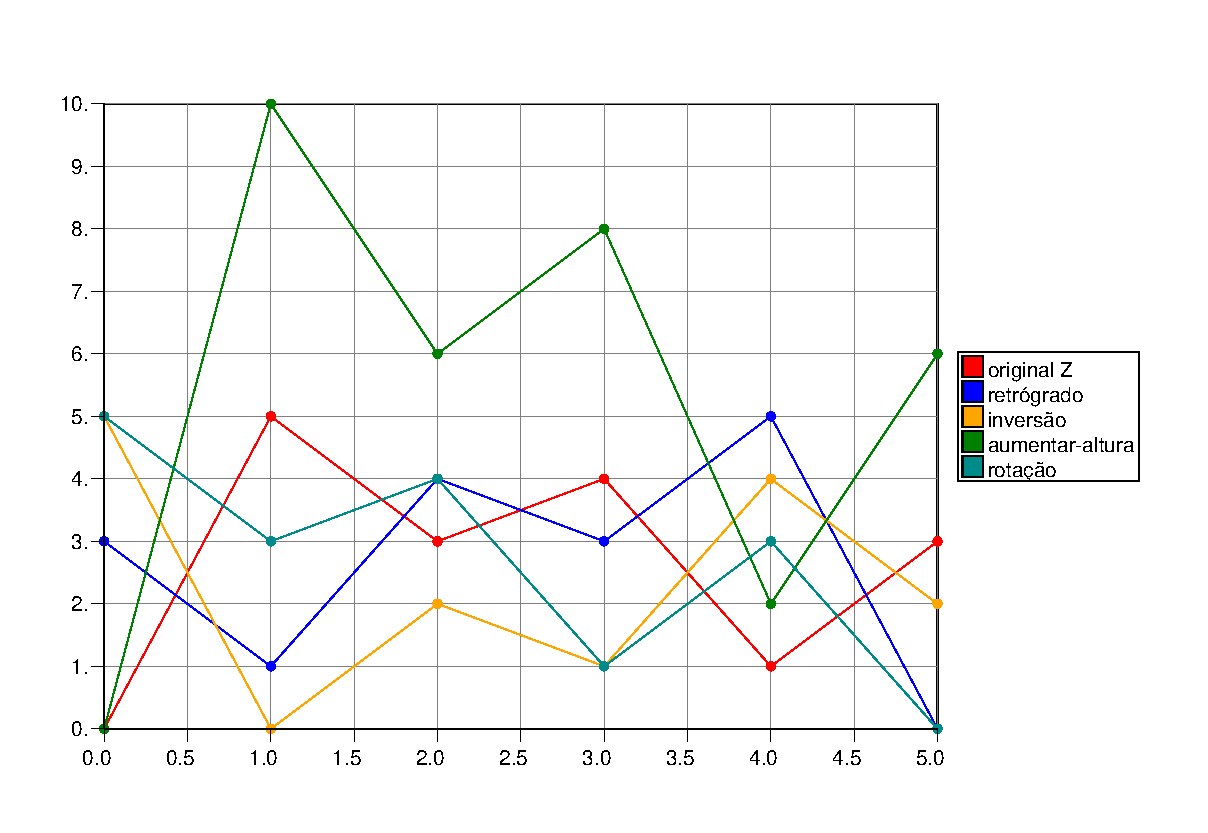
\includegraphics[scale=.5]{contornos}
  \caption{Operações em contorno (0 5 3 4 1 3)}
  \label{fig:operacoes}
\end{figure}
Para o futuro pretendemos implementar a possibilidade de gerar
contornos a partir de partituras musicais e vice-versa e implementar
uma interface gráfica. O desenvolvimento do \goiaba{} segue
procedimentos oriundos do desenvolvimento de software livre como uso
de controle de versão e disponibilização do código-fonte na
internet\footnote{Disponível como marcos-mestrado.git em
  \url{git.genos.mus.br}.}.

As descrições das teorias de contornos nem sempre são feitas pelos
seus autores de uma forma totalmente clara. A programação de uma
teoria em um software de computador é um exercício poderoso no
processo de aprendizagem, pois o programador é obrigado a expressar de
forma precisa a compreensão que tem de uma idéia obscura. Dessa forma
a implementação das operações de contorno em um software de computador
ajuda na compreensão da teoria, uma vez que é preciso entender
totalmente como cada operação se processa e que funcionalidade tem
para implementá-las.

As operações são implementadas como funções. Para isso é necessário
conhecê-las de modo profundo e abstraí-las precisamente em descrições
matemáticas. As funções têm que ser testadas a partir de aplicações
práticas. Para os testes são utilizados exemplos originais dos
autores, e são criados exemplos adicionais, o que ajuda na compreensão
da funcionalidade de cada operação. Finalmente combinações de funções
são observadas e testadas. Este processo de aprendizagem tem se
mostrado muito eficiente e se tornou fundamental para o
desenvolvimento da pesquisa.

\section{Outras ferramentas computacionais}
\label{sec:outr-ferr-comp}

Algumas das ferramentas utilizadas são aqui descritas porque, apesar
de serem amplamente utilizadas em outras áreas como ciência da
computação ou matemática, são praticamente desconhecidas entre
músicos.

\subsection{Lilypond}
\label{sec:lilypond}

O Lilypond\footnote{\url{www.lilypond.org}} é um software livre para
edição automática de partituras. É automático porque na maioria dos
casos dispensa ajustes como número de compassos por sistema, número de
sistemas por página, distância entre pentagramas, entre notas e
acidentes, entre outros.

O Lilypond processa música descrita em uma sintaxe própria de marcação
e gera arquivos como .pdf, .ps, .midi, .png, .svg entre outros. A
figura XXX por exemplo é gerada com um código como
\verb!{ \clef bass c4 d8 e d4 c }!. É possível utilizar variáveis para
abstrair códigos. Em Composição isso pode ser usado para abstrair
motivos, por exemplo. Dessa forma, um código como este:

\begin{verbatim}
{
  c4 e
  e16 d c d
  d4 fis
  e16 d c d
}
\end{verbatim}

pode ser escrito desta forma:

\begin{verbatim}
motivoA = { c4 e }
motivoB = { e16 d c d }
{
  \motivoA
  \motivoB
  \transpose c d {motivoA}
  \motivoB
}
\end{verbatim}

O Lilypond se relaciona com o \LaTeX{} de modo a simplificar a
produção de exemplos musicais para inserir em texto. Por fim é
possível desenvolver programas que usem o Lilypond para gerar
partitura automaticamente. O Rameau, por exemplo, faz análise
harmônica automática e gera como saída partitura através do Lilypond
\cite{kroger08:rameau}.

\subsection{Git}
\label{sec:git}

%% dizer o que é um sistema de controle de versão
Um sistema de controle de versão é um programa de computador que tem
como função gerenciar todas as versões de arquivos de um determinado
projeto. É normalmente utilizado em desenvolvimento de software,
embora seu uso não seja restrito a este tipo de atividade.

%% falar de funcionalidades de um sistema de controle de versão
Um sistema de controle de versão possibilita o trabalho colaborativo
sem conflitos entre as versões dos arquivos dos usuários. Com um
sistema deste é possível comparar versões de arquivos para observar as
mudanças, voltar a versões antigas para encontrar erros, criar novos
ramos paralelos de desenvolvimento e outras inúmeras funcionalidades.

%% explicar em linhas gerais como um sistema de controle de versão funciona
Normalmente inicia-se o controle de versão no diretório raiz de um
projeto. O sistema cria um repositório oculto para onde todos os
arquivos e mudanças colocados em controle de versão são copiados. O
procedimento do usuário normalmente é salvar cada mudança feita em um
arquivo com um título e descrição, de forma que ele possa reconhecer a
mudança quando precisar. A figura \ref{fig:controle-de-versao} mostra
um esquema gráfico deste processo. Neste exemplo o arquivo foo é
alterado e a linha com o texto \verb!43! é substituída por
\verb!43 MS!. O sistema compara a versão do diretório com a versão do
repositório e salva apenas as mudanças. O esquema de funcionamento
interno dos repositórios é diferente em cada sistema de controle de
versão, embora o processo para o usuário seja sempre parecido com o
que apresentamos.

\begin{figure}
  \centering
  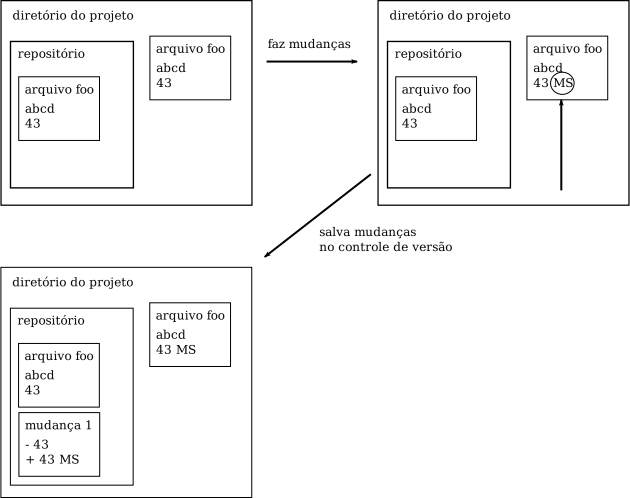
\includegraphics[scale=.6]{controle-de-versao}
  \caption{Funcionamento de um sistema de controle de versão}
  \label{fig:controle-de-versao}
\end{figure}

%% desenvolver sobre git
O Git\footnote{\url{http://git.or.cz}}---\eng{Fast Version Control
  System}---é um software livre de controle de versão bastante
poderoso e veloz. Como outros sistemas modernos, permite o
desenvolvimento distribuído, em que cada desenvolvedor pode ter uma
cópia local do repositório central, que fica acessível via
SSH\footnote{Protocolo de acesso remoto seguro} ou HTTP. O Git tem
suporte a desenvolvimento não-linear com ramos, ou seja, é possível
desenvolver uma nova versão de um programa ao mesmo tempo em que
defeitos da versão anterior são corrigidos. Com o Git é possível
trabalhar com grandes projetos e ter velocidade de processamento muito
maior que outros sistemas de controle de versão. O Git proporciona
segurança do histórico de mudanças. Uma vez que uma mudança é
registrada ela pode ser revertida, mas não pode ser removida do
histórico, ou seja, é possível saber tudo que foi feito em um
projeto. Finalmente o Git oferece um conjunto de ferramentas de fácil
utilização para gerenciar o projeto. A figura \ref{fig:historico-git}
mostra uma interface gráfica do Git para visualizar histórico de
mudanças, autor, data e hora da mudança, arquivos alterados e a
alteração em si.

\begin{figure}
  \centering
  \includegraphics[scale=.5]{gitk}
  \caption{Visualização de histórico do projeto no Gitk}
  \label{fig:historico-git}
\end{figure}

%% falar sobre controle de versão neste trabalho (programa, projeto,
%% composições e dissertação)
Utilizamos o sistema de controle de versão Git no desenvolvimento de
todo o trabalho. Mantivemos este projeto em um repositório
central\footnote{Disponível em
  \url{git.genos.mus.br/marcos-mestrado.git}.} com acesso irrestrito
ao autor e orientador. Este procedimento dinamizou muito o trabalho
uma vez que todo e qualquer comentário ou modificação pôde ser feita
diretamente no texto sem necessidade de um aviso prévio. O sistema de
controle de versão foi suficiente para registrar dados como mudança e
autoria. Usamos controle de versão no gerenciamento do desenvolvimento
do Goiaba, nos experimentos composicionais, na obra final, e na
escrita desta dissertação e do seu projeto.

A possibilidade de criar ramos diferentes de desenvolvimento nos
possibilitou fazer a refatoração do Goiaba ao mesmo tempo que podíamos
ter em funcionamento uma versão estável anterior.

Na composição o sistema possibilitou, por exemplo, consultas
posteriores a fragmentos que havíamos desistido de manter na obra. Com
um sistema deste tipo é possível reconstituir o passo-a-passo do
compositor na criação de uma obra musical.

A produção desta dissertação ilustra o uso de controle de versão em um
projeto colaborativo. Em um trabalho sem este tipo de ferramenta,
enquanto o orientador faz notas no texto, o autor não pode editá-lo
para não criar conflitos entre as versões. Neste trabalho pudemos
trabalhar sempre simultaneamente.


\chapter{Análise da obra \obra{}}
\label{cha:anal-da-obra}
%% falar de contornos, motivos, forma, altura, timbre, gestual

A obra \obra{} é um quinteto de madeiras em movimento único. Sua
composição foi focada no uso sistemático de contornos melódicos e
não-melódicos. Além de contornos, trabalhamos com proporções, metas
composicionais, gestos e motivos em um nível secundário.

A obra contém três elementos musicais a partir dos quais todo o
material composicional é derivado. O primeiro elemento é uma estrutura
de duas vozes---representada pela figura \ref{fig:bifonia}. O segundo
elemento é o motivo $\alpha$\footnote{Os motivos são descritos na
  seção \ref{sec:uso-de-motivos}.}, o principal da obra, representado
pela figura \ref{fig:motivo-alfa}. Este motivo é derivado por meio de
alternância entre as notas da estrutura de duas vozes. O terceiro
elemento é o contorno principal da peça \contpr{}, representado pela
figura \ref{fig:534120}. Este é o contorno do motivo $\alpha$.

\begin{figure}
  \centering
  \subfloat [Estrutura de duas vozes]{
    \includegraphics{bifonia}
    \label{fig:bifonia}
  }
  \subfloat [Motivo $\alpha$]{
    \includegraphics{motivo-alfa}
    \label{fig:motivo-alfa}
  }

  \subfloat [Representação gráfica do contorno (5 3 4 1 2 0)]{
    \includegraphics{c-534120}
    \label{fig:534120}
  }
  \caption{Elementos geradores}
  \label{fig:elementos-geradores}
\end{figure}

\section{Aspectos formais}
\label{sec:aspectos-formais}

Esta obra pode ser dividida em sete seções. Cada uma destas seções
contém uma textura característica, um desenho gestual e uma meta
composicional.
%% reescrever período
O tamanho de cada seção foi definido no planejamento inicial da obra
com proporções baseadas na razão áurea.
%%
Porém, como admitimos uma tolerância relativamente alta entre
planejamento e resultado final, estas proporções ficaram diferentes na
versão final da obra.
%% dizer o quanto desviei
Admitimos esta alta tolerância porque decidimos concentrar esforços no
objetivo principal do trabalho e deixar questões como proporções
formais em segundo plano.

A tabela \ref{tab:secoes-obra} contém informações de cada uma das
seções da obra como a duração, andamento, a localização do seu início
e fim pelo número de compasso e letra de ensaio.

\begin{table}
  \centering
  \begin{tabular}{r|ccccccc}
    Seção & 1 & 2 & 3 & 4 & 5 & 6 & 7 \\
    \hline
    Início (letra ensaio) & - & E & H & L & O & R & U \\
    Início (comp.) & 1 & 37 & 57 & 105 & 134 & 173 & 215 \\
    Final (comp.) & 36 & 56 & 104 & 133 & 172 & 214 & 244 \\
    Duração aprox. (s) & 132 & 91 & 108 & 56 & 87 & 23 & 16\\
    Andamento M.M & 82 & 66 & 120 & 120 & 108 & 112 & 112 \\
  \end{tabular}
  \caption{Seções formais da obra}
  \label{tab:secoes-obra}
\end{table}

\subsection{Planejamento da composição}
\label{sec:plan-da-comp}

O planejamento inicial desta peça foi feito pouco menos de um ano
antes de sua composição. Neste planejamento detalhamos elementos de
alto nível de abstração como forma, seções, microseções, proporções,
andamentos, metas composicionais e texturas. Consideramos estruturas
musicais como temas, movimentos, seções como de alto nível de
abstração, e notas e durações como de baixo nível de abstração. O
resultado deste planejamento pode ser visto na tabela
\ref{tab:planejamento-inicial}. Muitos dos elementos planejados foram
modificados em função da própria dinâmica da composição. À medida que
a música foi criada adaptamos o planejamento privilegiando o resultado
artístico.

\begin{table}
  %% aumentar a fonte das palavras
  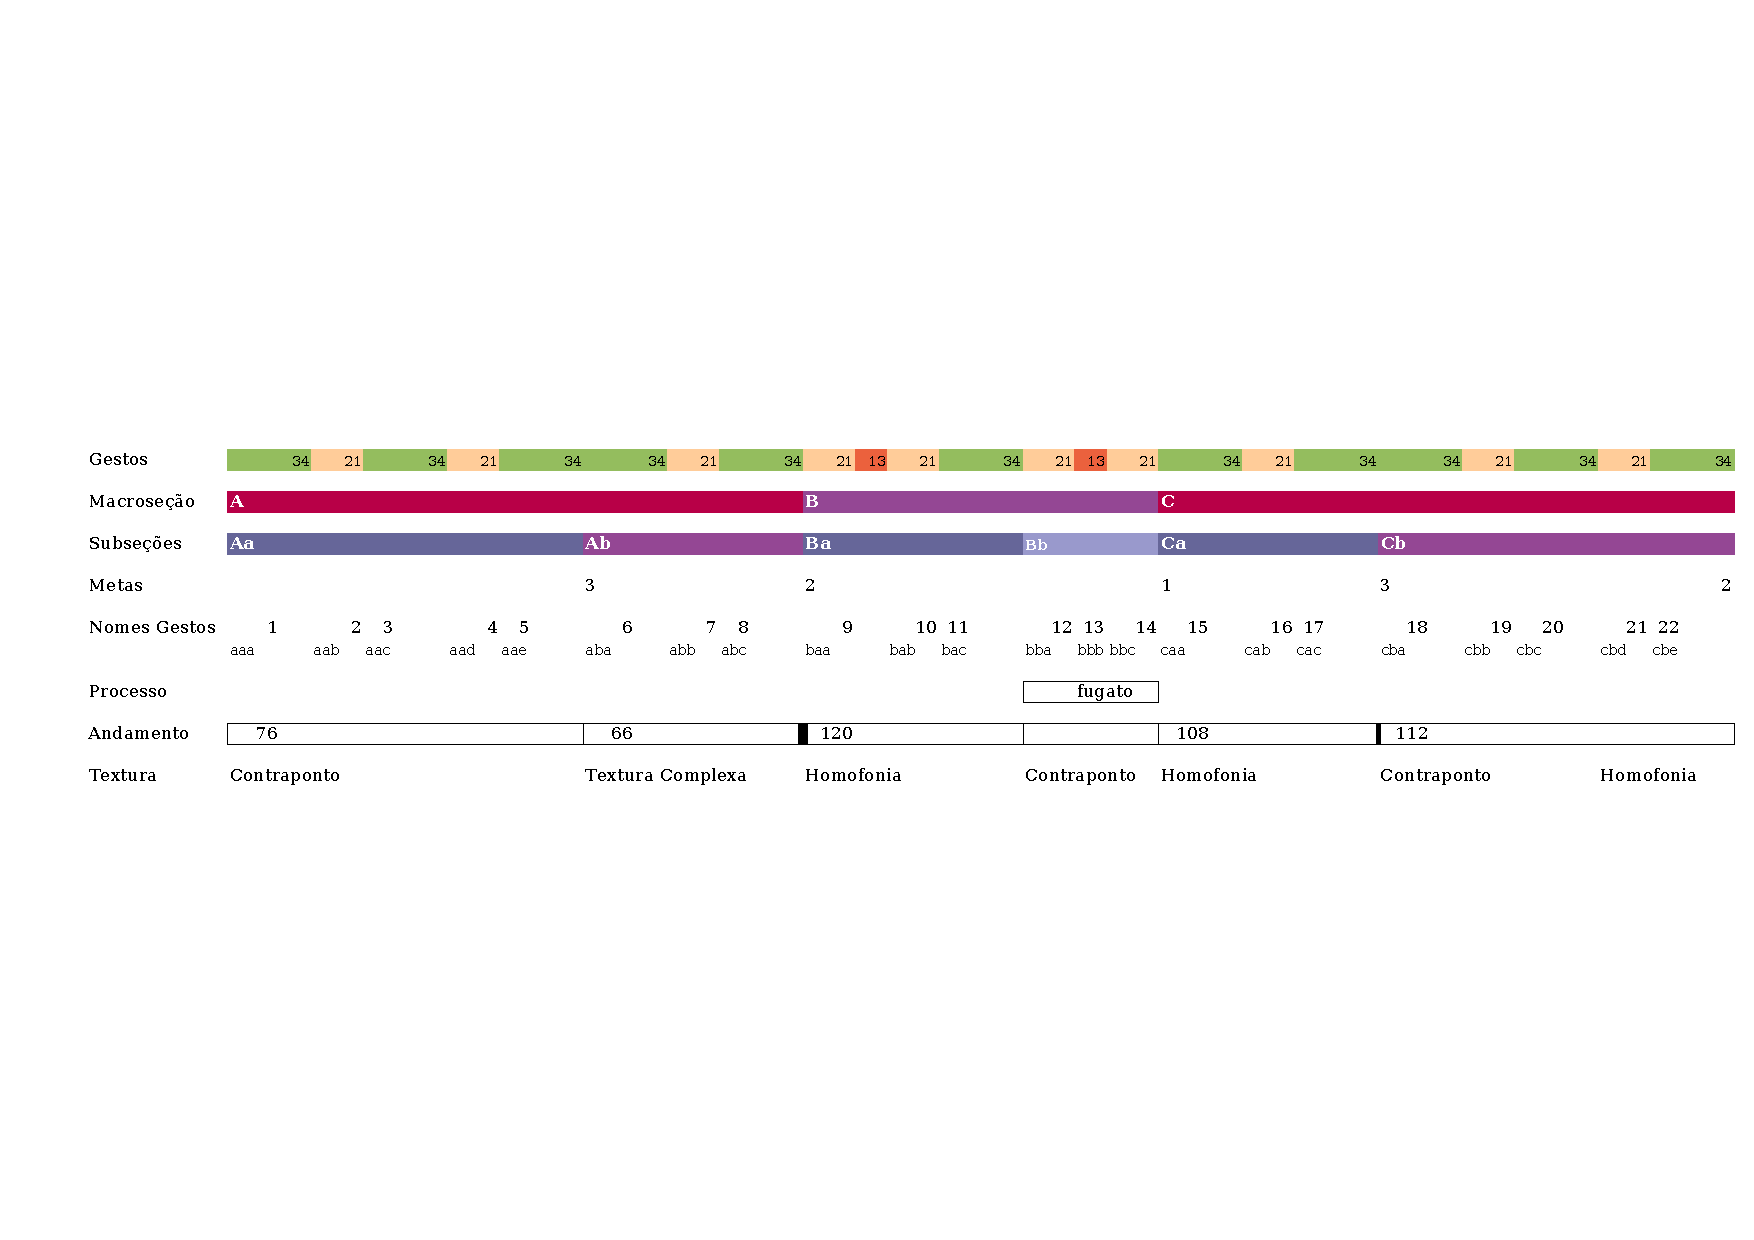
\includegraphics[scale=.81]{planejamento-inicial}
  \caption{Planejamento inicial da peça}
  \label{tab:planejamento-inicial}
\end{table}

No planejamento previmos criar seis seções agrupáveis duas a duas (Aa,
Ab, Ba, Bb, Ca, Cb). Durante a composição dividimos a seção Cb em dois
pedaços, criando então uma nova seção.

As seções menores estão desmembradas em sub-seções (Aaa, Aab, Aac e
assim por diante). Estas divisões mínimas foram planejadas para conter
microgestos, mas ao longo do processo preferimos trabalhar com gestos
maiores e usá-las para marcar mudanças de instrumental, de timbre, ou
outras intervenções musicais. Além disso os nomes e as numerações dos
gestos ajudaram na organização dos arquivos do Lilypond durante a
composição.

O uso destas microseções para mudança de instrumental pode ser visto
na seção inicial da peça (vide tabela
\ref{tab:microsecoes-primeira-secao}). A microseção \textbf{Aaa}
(compassos 1--8) compreende o solo do fagote e tem 29 segundos. a
microseção \textbf{Aab} (compassos 9--14) compreende o trio entre
fagote, clarinete e oboé e tem 22 segundos. A microseção \textbf{Aac}
(compassos 15--22), de 29 segundos compreende o duo entre a melodia
inicial no clarinete e o contraponto da flauta. A microseção
\textbf{Aad} (compassos 23--28), de 22 segundos compreende o quinteto
completo. Por último, a microseção \textbf{Aae} (compassos 29--36), de
29 segundos, compreende o quarteto fl./ob./cal./fg. e o aumento da
densidade.

\begin{table}
  \centering
  \begin{tabular}{r|rrrrr}
    & Aaa & Aab & Aac & Aad & Aae \\
    \hline
    Flauta & & & \cinzaa & \cinzaa & \cinzaa \\
    Oboé & & \cinzab & & \cinzab & \cinzab \\
    Clarinete & & \cinzaa & \cinzaa & \cinzaa & \cinzaa \\
    Trompa & & & & \cinzaa & \cinzaa \\
    Fagote & \cinzab & \cinzab & & \cinzab &
  \end{tabular}
  \caption{Instrumentos utilizados na primeira seção}
  \label{tab:microsecoes-primeira-secao}
\end{table}

%% explicar melhor este período:
Os números 1, 2 e 3 associados às metas representam seu grau de
importância na peça.
%% verificar: gradação ou graduação
Tal graduação porém não foi implementada. Os andamentos foram
levemente modificados para adequação ao material de cada seção. Na
tabela \ref{tab:planejamento-inicial} as barras mais grossas nos
campos dos andamentos representam silêncio entre as seções e não foram
implementadas na versão final. As texturas planejadas foram mantidas
exceto pela seção planejada C (seções 5--7). Neste ponto não há de
fato textura homofônica.

\subsection{Descrição das seções}
\label{sec:descricao-das-secoes}

A seção 1, no início da obra\footnote{Vide seções na tabela
  \ref{tab:secoes-obra}.}, contém em toda sua extensão a repetição de
uma mesma melodia (figura \ref{fig:melodia-inicial}). Esta repetição é
alternada entre os instrumentos. Ainda nesta seção, a partir do
compasso 9, o motivo $\alpha$ (figura \ref{fig:motivo-alfa}) aparece
simultaneamente em duas vozes formando uma textura contrapontística
(figura \ref{fig:contraponto-alfa}). O progressivo aumento da
densidade e do nível de dinâmica colaboram com o desenho gestual da
seção, que culmina no acorde do compasso 36.

\begin{figure}
  \centering
  \includegraphics{melodia-inicial}
  \caption{Melodia inicial}
  \label{fig:melodia-inicial}
\end{figure}

\begin{figure}
  \centering
  \includegraphics{contraponto-alfa}
  \caption{Contraponto com motivo $\alpha$}
  \label{fig:contraponto-alfa}
\end{figure}

A seção 2 contém uma textura de entradas defasadas de notas longas. O
seu gestual forma um arco em que a densidade aumenta até um pico, no
compasso 47, e gradativamente decresce. A variação de densidade é
obtida com a variação de amplitude (representada na figura
\ref{fig:amplitude-secao-2}) e com o estreitamento e alargamento das
entradas instrumentais. A variação de amplitude está associada à
expansão e contração de intervalos entre as notas (vide redução das
notas na figura \ref{fig:notas-secao-2}).

\begin{figure}
  \centering
  \includegraphics[scale=.7]{amplitude-secao-2}
  \caption{Representação da amplitude na seção 2 em \eng{piano roll}}
  \label{fig:amplitude-secao-2}
\end{figure}

\begin{figure}
  \centering
  \includegraphics{secao-2}
  \caption{Redução analítica da seção 2---notas}
  \label{fig:notas-secao-2}
\end{figure}

A seção 3 compreende uma textura de melodia principal e
acompanhamento. A sua textura contém três elementos que podem ser
vistos na figura \ref{fig:textura-secao-3}: a) linha com notas de
articulação stacattíssimo atacadas nos tempos 1 e 2 (trompa); b) linha
com notas de articulação stacatto repetidas nas partes fracas do tempo
(fagote); c) melodia principal (clarinete). O elemento ``a'' é
apresentado com as notas lá e sol, o elemento ``b'' com as notas lá,
sol, dó$\sharp$ e ré$\sharp$, e o elemento ``c'' é apresentado com as
notas do motivo $alpha$ (figura \ref{fig:motivo-alfa}) com e sem
transposição para mi. O gestual da seção delineia um gradual aumento
de densidade e direcionamento para o agudo e culmina no início da
seção 4.

\begin{figure}
  \centering
  \includegraphics{textura-secao-3}
  \caption{Textura da seção 3}
  \label{fig:textura-secao-3}
\end{figure}

O início da seção 4 ocorre antes do final da seção 3, que tem um
desfecho gradativo, formando uma espécie de dégradé entre estas seções
(figura \ref{fig:transicao-secao-3-4}). A seção 4 é um fugato com sujeito e
contra-sujeito derivados do contorno principal e de combinações de
operações\footnote{Para maiores detalhes sobre este fugato e
  combinações de operações vide seção \ref{sec:comb-de-oper}.}. Do
ponto de vista gestual, há uma passagem de uma menor densidade no
início da seção 4, com as entradas instrumentais sucessivas, para uma
maior densidade no final da mesma seção. Isto ocorre por três razões:
(1) a entrada da trompa em ritmo largo (comp. 123), (2) o
estreitamento entre as entradas das madeiras, e (3) a partir do
compasso 128, o jogo de perguntas e respostas com o primeiro segmento
do sujeito, que ocorre entre as duplas flauta/fagote e oboé/clarinete.

\begin{figure}
  \centering
  \includegraphics{transicao-secao-3-4}
  \caption{Transição entre seções 3 e 4}
  \label{fig:transicao-secao-3-4}
\end{figure}

A seção 5 tem como elemento fundamental um ostinato na linha do fagote
(figura \ref{fig:ostinato-fagote}). Este ostinato é inspirado em um
dos toques da capoeira\footnote{A utilização deste elemento foi apenas
  pontual. Por este motivo não aprofundaremos em maiores explicações
  sobre a capoeira e seus toques.}. O ritmo do ostinato é aproveitado
para a construção da estrutura de duas vozes (vide seção
\ref{sec:aspectos-verticais}). O desenho gestual desta seção é
bastante parecido ao da seção 1, com aumento progressivo da densidade
culminando no acorde do compasso 172.

\begin{figure}
  \centering
  \includegraphics{ostinato-fagote}
  \caption{Ostinato da linha do fagote}
  \label{fig:ostinato-fagote}
\end{figure}

A seção 6, em contraste às anteriores, é caracterizada por grupos de
notas curtas, rápidas e desligadas. Estes grupos são separados entre
si por silêncios (figura \ref{fig:sexta-secao-184-187}). As linhas dos
instrumentos contêm cada uma o motivo $\alpha$ modificado por
operações de rotação\footnote{Estas operações estão descritas na seção
  \ref{sec:comb-de-oper}.}. Os grupos de notas curtas não englobam
necessariamente todas as notas do motivo $\alpha$. Por vezes o
silêncio interrompe o motivo, como por exemplo na linha da flauta, nos
compassos 177--178 (figura \ref{fig:grupos-separados-silencio}). O
motivo é concluído logo após o silêncio.

\begin{figure}
  \centering
  \subfloat[Textura de notas curtas e silêncios (em dó)]{
    \includegraphics{sexta-secao-184-187}
    \label{fig:sexta-secao-184-187}
  }

  \subfloat[Motivo interrompido por silêncio]{
    \includegraphics{flauta-grupos-silencio}
    \label{fig:grupos-separados-silencio}
  }

  \subfloat[Transição entre os dois gestos da seção 6]{
    \includegraphics{transicao-sexta-dois-gestos}
    \label{fig:transicao-sexta-dois-gestos}
  }
  \caption{Notas curtas separadas por silêncios (seção 6)}
  \label{fig:sexta-secao-notas-curtas}
\end{figure}

A seção 6 contém dois gestos interligados. O primeiro gesto
(comp. 173--198) é marcado pelo aumento da densidade, obtido pela
diminuição dos silêncios. O colorido melódico tem destaque no final
deste gesto (comp. 194--198). O segundo gesto (comp. 199--214) é
caracterizado por graduais movimentos ascendentes e movimentação do
âmbito do grave para o agudo. A linha da trompa (comp. 206--215),
derivada da linha do oboé (comp. 149--157) interliga esta seção com a
seguinte. Na figura \ref{fig:transicao-sexta-dois-gestos} percebemos o
início do segundo gesto com elementos do gesto anterior.

A seção 7, última da obra, engloba elementos importantes das seções
anteriores (figura \ref{fig:setima-secao-resumo}). A linha do fagote é
uma repetição do que ocorre na seção 4. A linha do clarinete
representa o ritmo e acentuação da seção 3. A linha da trompa
corresponde ao solo do fagote do início da peça. As linhas do oboé e
flauta representam a estrutura de duas vozes apresentada na seção
5. Finalmente o material apresentado pela flauta e oboé a partir do
compasso 239 representa o sujeito do fugato da seção 4. As relações de
contornos nesta seção são, portanto, as mesmas que estes citados
elementos mantêm nas seções anteriores.

\begin{figure}
  \centering
  \includegraphics{setima-secao-resumo}
  \caption{Elementos de outras seções na seção 7}
  \label{fig:setima-secao-resumo}
\end{figure}
\section{Aspectos verticais}
\label{sec:aspectos-verticais}
%% aspectos "harmônicos". melhorar título da seção

A estrutura de duas vozes (figura \ref{fig:bifonia},
p. \pageref{fig:bifonia}) que origina todo material da peça tem seu
conteúdo harmônico derivado da escala octatônica\footnote{A escala
  octatônica é obtida a partir da superposição de duas das três
  tétrades diminutas contidas em uma escala dodecafônica
  \cite[p. 76]{antokoletz90:music}.} (figura
\ref{fig:escala-octatonica}).

\begin{figure}
  \centering
  \includegraphics{escala-octatonica}
  \caption{Escala octatônica}
  \label{fig:escala-octatonica}
\end{figure}

Ao longo da obra um acorde é apresentado de forma recorrente (figura
\ref{fig:acorde-motivo}). Este acorde é derivado da estrutura de duas
vozes e tem sonoridade octatônica. A seção 3 é inteiramente construída
com este acorde, que tem sua orquestração modificada no decorrer do
gesto.

\begin{figure}
  \centering
  \includegraphics{acorde-motivo}
  \caption{Acorde-motivo}
  \label{fig:acorde-motivo}
\end{figure}

A estrutura de duas vozes é apresentada em sua forma mais explícita na
seção 5 (figura \ref{fig:bifonia-grave}). Aparece inicialmente na
região grave, nas linhas do clarinete e da trompa (comp. 137--144),
depois brevemente no oboé e na trompa (comp. 146--149), e mais adiante
na flauta e no clarinete (comp. 157--172).

\begin{figure}
  \centering
  \includegraphics{bifonia-grave}
  \caption{Apresentação da estrutura de duas vozes no clarinete e
    trompa (ambos em dó) c. 137--141}
  \label{fig:bifonia-grave}
\end{figure}
\section{Uso de motivos}
\label{sec:uso-de-motivos}

A obra contém três motivos derivados da estrutura de duas vozes
(figura \ref{fig:bifonia}, p. \pageref{fig:bifonia}). O motivo
$\alpha$ (figura \ref{fig:motivo-alfa-analisado}) dá origem aos
motivos de três notas $\beta$ (figura \ref{fig:motivo-beta}) e de
semicolcheias $\gamma$ (figura \ref{fig:motivo-gama}). Além destes há
a presença de um motivo unicamente rítmico $\delta$ (figura
\ref{fig:motivo-delta}).

\begin{figure}
  \centering
  \subfloat[Motivo $\beta$]{
    \includegraphics{motivo-beta}
    \label{fig:motivo-beta}
  }
  \subfloat[Motivo $\gamma$]{
    \includegraphics{motivo-gama}
    \label{fig:motivo-gama}
  }

  \subfloat[Motivo $\delta$]{
    \includegraphics{motivo-delta}
    \label{fig:motivo-delta}
  }

  \subfloat[Estrutura do motivo $\alpha$]{
    \includegraphics{motivo-alfa-analisado}
    \label{fig:motivo-alfa-analisado}
  }
  \caption{Motivos utilizados na obra}
  \label{fig:motivos-utilizados}
\end{figure}

O motivo $\alpha$ contém dois motivos $\beta$, um em sua forma
original e outro invertido. Além disso o motivo $\alpha$ também está
presente de forma invertida no motivo $\gamma$, com as notas
Dó-Mi$\flat$-Ré$\flat$. Este motivo $\alpha$ é utilizado na linha do
fagote do início da peça, no sujeito do fugato da seção 4 (letra L),
na linha do clarinete nos compassos 137--144, na linha da flauta nos
compassos 158--171, no material da flauta e oboé na seção 6 (letra R)
e na seção final.
%% inserir figura com linha inicial do fagote
%% inserir seção em que falo que a última seção é resumo das outras

O motivo $\gamma$ é exatamente um retrógrado do motivo $\alpha$ com a
adição do parâmetro duração e da característica anacrúzica. O motivo
está presente na linha do oboé, compasso 149, nas linhas da flauta e
clarinete nos compassos 157--172, na contrução do material ascendente
dos compassos 200--215 e na seção final.

O motivo $\delta$ não tem relação com altura ou contorno. É apenas um
padrão de acentuação que é repetido nas seções 3 e 7. Na primeira
aparição há notas \eng{stacatto} entre os acentos. Na segunda aparição
há apenas os acentos.

\section{Uso de contornos}
\label{sec:uso-de-contornos}

O objetivo principal da composição da obra \obra{} foi o uso
sistemático de combinações de operações de contorno para a criação
musical. Por isso decidimos escolher um único contorno---de modo a
colaborar com a unidade da peça---e manipulá-lo para gerar a maioria
do material composicional da obra. Escolhemos o contorno de seis
elementos \contpr{}, relacionado com a estrutura de duas vozes e o
motivo $\alpha$.

O contorno principal \contpr{} tem forma prima c6-26 (0 2 1 4 3
5)\footnote{A numeração dos contornos (ou segmentos de contornos) pode
  ser vista na Tabela de classes de segmentos de contornos
  \cite{marvin.ea87:relating}.}. Este é um contorno simétrico, por
isso retrógrado e inversão são iguais. Este contorno contém
subconjuntos de 5, 4, 3 e 2 elementos.

\subsection{Combinações de operações de contorno utilizadas}
\label{sec:comb-de-oper}

Utilizamos um grupo de operações de contorno e as combinamos para
criar o material musical da obra. Trabalhamos com dois subconjuntos de
contornos, operações de INT$_1$, inversão, rotações e de preenchimento
de contornos. Combinamos estas operações desta forma:

\begin{itemize}
\item Subconjunto com expansão e transposição
\item Interpolação com expansão
\item Rotação com expansão
\item Concatenação de contornos resultando em novo material
\item Rotação com retrogradação
\end{itemize}

%% dúvida: que termo devo usar em relação à linha do fagote? melodia?
%% fragmento melódico? motivo?

%% kroger: talvez "solo de fagote" se voce esta se referindo apenas ao
%% solo de fagote (antes dos instrumentos entrarem) :-)

%% marcos: estou preferindo deixar "melodia"

A combinação das operações de subconjunto, expansão e transposição foi
utilizada na linha do fagote no início da peça. Neste ponto há uma
melodia (figura \ref{fig:melodia-inicial},
p. \pageref{fig:melodia-inicial}) construída com o subconjunto do
contorno principal (2 0 1). A melodia tem dois segmentos, sendo o
primeiro derivado das três notas iniciais do motivo $\alpha$, e o
segundo como transposição do segmento anterior com operações de
expansão e transposição. Em ambos os segmentos há preservação do
contorno (2 0 1). Esta melodia está presente em toda a primeira seção
da obra, nos compassos 9--14 no fagote e oboé, nos compassos 15--22 no
clarinete, e nos compassos 23--36 na flauta e trompa.

A combinação de rotação e expansão de contornos ocorre no sujeito e
contra-sujeito do fugato da seção 4 e no material de notas curtas da
seção 6. O sujeito do fugato (figura \ref{fig:sujeito-fugato}) é
constituído por dois segmentos elididos. O primeiro segmento é o
próprio motivo $\alpha$, por consequüencia, é também o contorno
principal (5 3 4 1 2 0). O segundo segmento é o contorno resultante da
combinação da operação de rotação de fator 3, (1 2 0 5 3 4), e da
operação de expansão. O segundo segmento é iniciado na nota Sol,
última nota do segmento anterior.

O contra-sujeito é composto de três segmentos que contêm combinações
de operações de retrogradação e rotação de contornos (figura
\ref{fig:contra-sujeito-fugato}). O primeiro segmento contém uma
rotação de fator 5 do retrógrado do contorno principal (5 0 2 1 4
3). A primeira nota está elidida com a última nota do sujeito. O
segundo segmento contém uma rotação de fator 4 do retrógrado do
contorno principal (3 5 0 2 1 4), e também está elidida ao segmento
anterior. Finalmente o terceiro segmento contém uma rotação de fator 3
do retrógrado do contorno principal (4 3 5 0 2 1). Ao contrário dos
outros segmentos, ele não está elidido ao segmento anterior. Pode-se
observar que o contra-sujeito incorpora ainda uma sistemática nas suas
operações de contorno. A cada segmento o fator de rotação diminui em
um ponto.

\begin{figure}
  \centering
  \subfloat[Sujeito]{
    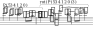
\includegraphics{sujeito-fugato}
    \label{fig:sujeito-fugato}
  }

  \subfloat[Contra-Sujeito]{
    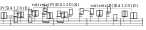
\includegraphics{contra-sujeito-fugato}
    \label{fig:contra-sujeito-fugato}
  }
  \caption{Elementos estruturais do fugato}
  \label{fig:elementos-fugato}
\end{figure}

A combinação de rotação e expansão de contornos também está presente
na seção 6, nas linhas das quatro madeiras. A linha da flauta contém o
motivo $\alpha$ em sua forma original. A linha do clarinete contém uma
rotação de fator 2 e uma expansão de intervalos de segunda para
intervalos de terça. A linha do oboé contém um desvio da estrutura do
contorno. Trata-se de uma rotação de fator 3 do motivo $\alpha$, porém
com transposição da segunda metade do motivo para uma oitava
abaixo. Neste ponto a estrutura do contorno foi sacrificada em prol do
desenho gestual da seção, que não supera o Ré$\sharp$4 neste
trecho. Finalmente a linha do fagote contém uma rotação de fator 4 do
motivo $\alpha$ e expansão semelhante ao do clarinete. Na figura
\ref{fig:notas-curtas-madeiras} estão exibidas estas variações do
motivo $\alpha$ em cada elemento, na tabela
\ref{tab:operacoes-secao-6} há um esquema com as operações utilizadas
nestas variações, e na figura \ref{fig:rotacoes-534120} estão
representações gráficas das rotações utilizadas.

\begin{figure}
  \centering
    \includegraphics{notas-curtas-madeiras}
    \caption{Operações de rotação e expansão do motivo $\alpha$ na 6ª
    seção}
  \label{fig:notas-curtas-madeiras}
\end{figure}

\begin{figure}
  \centering
  \subfloat[Rotação 2: (4 1 2 0 5 3)]{
    \includegraphics{c-412053}
    \label{fig:412053}  
  }
  \subfloat[Rotação 3: (1 2 0 5 3 4)]{
    \includegraphics{c-120534}
    \label{fig:120534}  
  }
  \subfloat[Rotação 4: (2 0 5 3 4 1)]{
    \includegraphics{c-205341}
    \label{fig:205341}  
  }
  \caption{Rotações no contorno (5 3 4 1 2 0)}
  \label{fig:rotacoes-534120}
\end{figure}

\begin{table}
  \centering
  \begin{tabular}{r|cc}
    Instrumento & Fator de rotação & Expansão \\
    \hline
    Flauta & 0 & Não \\
    Oboé & 3 & Não \\
    Clarinete & 2 & Sim \\
    Fagote & 4 & Sim \\
  \end{tabular}
  \caption{Operações na seção 6}
  \label{tab:operacoes-secao-6}
\end{table}

A combinação entre expansão e retrogradação ocorre na linha do oboé
nos compassos 149--157 (figura \ref{fig:oboe-solo-secao-5}). O motivo
$\gamma$ (vide seção \ref{sec:uso-de-motivos} e figura
\ref{fig:motivo-gama}) é uma retrogradação do motivo $\alpha$ da
peça. Neste trecho este motivo aparece três vezes: na primeira vez em
sua forma original, na segunda vez com uma expansão e intervalo de
segunda para intervalo de terça, e na terça com uma expansão de
intervalo de segunda para intervalo de quarta.

%% inserir análise no inkscape
\begin{figure}
  \centering
  \includegraphics{oboe-solo-secao-5}
  \caption{Solo do oboé na seção 5}
  \label{fig:oboe-solo-secao-5}
\end{figure}

A combinação entre expansão, rotação, retrógrado e interpolação de
contornos ocorre na linha do oboé nos compassos 149--153. O motivo
$\alpha$ tem uma rotação de fator 3 gerando as notas adjacentes
Sol-Si$\flat$-Lá, e logo após, no compasso 152,
Dó$\sharp$-Si$\sharp$-Ré$\sharp$. Entre estes dois grupos de notas há
uma expansão de intervalos do motivo $\gamma$, iniciado em Dó$\sharp$3
e concluído em Dó$\sharp$4. Como já foi dito, este motivo é uma
retrogradação do motivo $\alpha$. Entendemos que este motivo está
interpolado com o contorno iniciado em Sol.

\subsection{Operações de contornos não combinadas}
\label{sec:cont-nao-comb}

A operação de INT$_1$ do contorno principal (- + - + -) ocorre de
maneira não ortodoxa no ostinato da linha do fagote, ao longo de toda
a seção 5 (figura \ref{fig:ostinato-fagote},
p. \pageref{fig:ostinato-fagote}). O padrão com as notas Sol e Lá
sugere o movimento (- +) presente no contorno principal.

A operação de expansão de intervalos também é usada de forma isolada
na segunda seção da obra. A expansão dos intervalos está associada à
omissão de notas da escala octatônica na construção do
contorno. Considerando-se a escala
Sol-Fá$\sharp$-Mi-Ré$\sharp$-Dó$\sharp$-Dó-Si$\flat$-Lá e omitindo-se
uma a cada duas notas, partindo-se de Sol tem-se
Sol-Mi-Dó$\sharp$-Si$\flat$. Omitindo-se duas a cada três notas tem-se
Sol-Ré$\sharp$-Si$\flat$ e assim por diante. O contorno é construído
com estas notas. A figura \ref{fig:escala-secao-2-one} mostra o
contorno com a omissão de uma a cada duas notas da escala octatônica,
e a figura \ref{fig:escala-secao-2-two} com a omissão de duas a cada
três notas da mesma escala.

\begin{figure}
  \centering
  \subfloat[Omissão de uma a cada duas notas]{
    \includegraphics[scale=1]{escala-secao-2-one}
    \label{fig:escala-secao-2-one}
  }

  \subfloat[Omissão de duas a cada três notas]{
    \includegraphics[scale=1]{escala-secao-2-two}
    \label{fig:escala-secao-2-two}
  }
  \caption{Expansão de intervalos por omissão de notas da escala
    octatônica}
  \label{fig:escala-secao-2}
\end{figure}

A operação de redução de contornos pode ser vista nas melodias
principais da seção 3 (figura \ref{fig:reducao-contornos-secao-3}). No
compasso 68 o contorno principal \contpr{} aparece na linha do
clarinete com apenas sua primeira e última notas (5 0). Nos compassos
76 e 81 o contorno aparece respectivamente nas linhas do oboé e
clarinete com apenas 4 notas. Na linha do oboé as notas centrais (4 1)
são omitidas para resultar no contorno (5 3 2 0), e na linha do
clarinete a segunda e penúltima notas (3 2) são omitidas para resultar
no contorno (5 4 1 0).

\begin{figure}
  \centering
  \subfloat[Nota inicial e nota final]{
    \includegraphics{reducao-contornos-secao-3-clarinete}
    \label{fig:reducao-contornos-secao-3-clarinete}
  }

  \subfloat[Omissão das duas notas centrais]{
    \includegraphics{reducao-contornos-secao-3-oboe}
    \label{fig:reducao-contornos-secao-3-oboe}
  }

  \subfloat[Omissão de duas notas intermediárias]{
    \includegraphics{reducao-contornos-secao-3-clarinete-2}
    \label{fig:reducao-contornos-secao-3-clarinete-2}
  }

  \caption{Redução de contornos na seção 3}
  \label{fig:reducao-contornos-secao-3}
\end{figure}

%% falar sobre o gestual da seção 5 e uso da anacruze e da
%% semelhança com o contraponto da primeira seção

\subsection{Contornos associados a outros parâmetros musicais}
\label{sec:cont-assoc-outr}

Contornos estão associados a outros parâmetros musicais como
andamento, densidade e textura.

Os andamentos utilizados na peça---82, 66, 120, 108 e 112 (vide tabela
\ref{tab:secoes-obra}, p. \pageref{tab:secoes-obra})---representam o
contorno A(1 0 4 2 3). Este contorno é um subconjunto de 5 elementos
do contorno principal utilizado, \contpr{}.

Na seção 1 relações de contornos estão associados a densidade. A
densidade neste trecho tem contorno D(1 3 2 5 4), isto é começa com um
instrumento, depois um trio, um duo, o quinteto completo e um
quarteto. Esta seção é iniciada com um solo de fagote (1) seguido de
um trio com fagote, clarinete e oboé (3). Ocorre então um duo entre
clarinete e flauta (2), um \eng{tutti} (5) e finalmente um quarteto
sem o fagote (4). Este contorno D é o retrógrado de um subconjunto de
5 elementos do contorno principal P.

As texturas presentes na peça podem ser divididas em dois grandes
grupos: de texturas homofônicas, que engloba texturas corais e de
melodia acompanhada; e de texturas polifônicas, que engloba textura
contrapontística e textura complexa. Estes grupos são apresentados
nesta ordem:
polifonia-homofonia-polifonia-homofonia-polifonia-homofonia. Considerando
que uma textura polifônica é mais complexa que uma textura homofônica,
a alternância entre estas texturas delineia um contorno de INT$_1$ (-
+ - + -), derivado do contorno principal \contpr{}.

\subsection{Operações de contorno não utilizadas}
\label{sec:oper-de-cont}

Nem todas as operações das teorias de contornos foram utilizadas na
composição. A matriz de comparação, por exemplo, é bastante utilizada para
análise, mas não encontramos uma forma interessante de usá-la na
composição.

\begin{figure}
  \centering
  \begin{tabular}{r|cccccc}
      & 5 & 3 & 4 & 1 & 2 & 0 \\
      \hline
    5 & 0 & - & - & - & - & - \\
    3 & + & 0 & + & - & - & - \\
    4 & + & - & 0 & - & - & - \\
    1 & + & + & + & 0 & + & - \\
    2 & + & + & + & - & 0 & - \\
    0 & + & + & + & + & + & 0
  \end{tabular}
  \caption{Matriz de comparação do contorno (5 3 4 1 2 0)}
  \label{fig:matriz-534120}
\end{figure}

\chapter{Partitura da obra \obra{}}
\label{cha:partitura-da-obra}

\input{paginas-composicao}

\chapter{Conclusão e discussão}
\label{cha:conclusao-e-discussao}

Contornos são estruturas musicais que podem efetivamente colaborar com
a coerência de uma obra musical. Teóricos desenvolveram operações de
comparação para análise musical algumas das quais podem ser utilizadas
na criação de material composicional, conforme mostrei ao longo deste
trabalho. Estas operações podem ser combinadas e resultar em uma maior
variedade de elementos derivados de um mesmo material gerador.

A obra \obra{} apresenta diversos usos de operações de contornos e
combinações. Toda obra foi desenvolvida a partir do contorno \contpr{}
e reuniu um grupo de operações e combinações derivadas de teorias de
contorno. Dessa forma este estudo contribui com a ampliação do estado
de arte de teorias de contorno incorporando possibilidades de
aplicações de operações de contorno na composição musical.

% Operações que "não funcionam" para composição

Algumas operações desenvolvidas para análise não pareceram funcionais
para a criação musical. A matriz de comparação por exemplo, embora
tenha sido intensamente usada por Morris, Marvin e Laprade não parece
ter um uso interessante para composição.

% operações "mais interessantes"

As operações mais interessantes para a composição foram expansão e
redução de intervalos, retrogradação, inversão, rotação, subconjuntos,
rotação e concatenação.

\section{Trabalhos futuros}
\label{sec:trabalhos-futuros}

A realização deste estudo abre caminho para vários outros trabalhos.

% Expansão do estudo: mapeamento de parâmetros em função de outros
% parâmetros além do tempo, survey

É importante fazer um mapeamento dos mais diversos parâmetros musicais
como dinâmica, densidade ou textura em função de outros parâmetros
além do tempo. Desta forma pode-se trabalhar com contornos como
dinâmica em função da densidade ou homogeneidade de timbre em função
da complexidade rítmica.

% Utilização de outras operações em composição.

É interessante testar outras operações das teorias de contornos em
composição compondo estudos de forma sistemática para testar cada
operação. Dessa forma é possível realmente saber como cada operação
pode ser utilizada na criação musical.

É importante compor estudos com instrumentos mais variados, como por
exemplo instrumentos sintetizados por computador. Este estudo pode
contribuir com os trabalhos de música computacional disponibilizando
contorno como elemento estruturador.

% Expansão do Goiaba

É necessário expandir o software Goiaba inserindo operações de todas
as teorias de contorno, acrescentando uma interface gráfica para que o
usuário possa clicar e arrastar pontos em um gráfico para gerar
contornos, inserindo funções para gerar partituras a partir de
contornos, e criando uma versão multiplataforma. Este estudo, além de
representar uma significativa ferramenta para a área de Composição,
pode incentivar compositores a usarem contornos de forma sistemática
em suas obras.

%%% Local Variables: 
%%% mode: latex
%%% TeX-master: "dissertacao-default"
%%% End: 